\section{Landing Phase}
\label{sec:landing_landing}
During landing, the character braces for impact, executes rolling
action, and gets up on its feet. Although these three stages take very
different actions, they share common control goals: modulating the COM
and posing important joints.  We apply the same control mechanism via
\emph{virtual forces} and \emph{PID joint-tracking} to produce the
final control forces for the forward simulator (Figure
\ref{fig:landing_landingOverview}).

\begin{figure}[htbp]
\center
  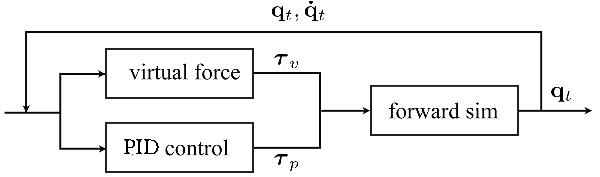
\includegraphics[width=3.2in]{images/landingOverview}
  \caption{Landing phase controller.}
 \label{fig:landing_landingOverview}
\end{figure}

Virtual forces are effective in controlling the motion of the COM. To
achieve a desired acceleration of the COM, $\ddot{\vc{c}}$, we compute
the virtual force as $\vc{f}_v = m \ddot{\vc{c}}$ where $m$ is the mass of the
character. The equivalent joint torque as if applying $\vc{f}_v$ to a
point $\vc{p}$ on the body is $\tau_v = \vc{J}^T (\vc{p}) \vc{f}_v$,
where $\vc{J}(\vc{p})$ is the Jacobian computed at the body point
$\vc{p}$.
If $\vc{p}$ is on a body node in contact with the ground, 
we apply the opposite force ($\vc{f}_v = -m \ddot{\vc{c}}$) in order to
generate a ground reaction force that pushes the COM in the desired direction.
To prevent the character from using excessively large joint
torques, we limit the magnitude of the sum of virtual forces.  A
successful landing motion also requires posing a few important joints
at each of the three stages. We track these partial poses with PID
servos: $\tau_p = k_p (\bar{q} - q) + k_i \int (\bar{q}_t - q_t) dt -
k_v \dot{q}$, where $k_p$, $k_i$ and $k_v$ are the proportional,
integral, and derivative gains respectively, and $\bar{q}$ is the
desired joint angle.  The final control torque is $\tau_v+\tau_p$.
We limit the magnitude of the virtual force to $3000N$ to prevent
excessive usage of joint torques.



\subsection{Impact Stage}
\label{sec:landing_impact}


Impact stage is the most critical stage during landing, which requires
careful control and execution. Human athletes tend to act like a
spring to absorb the effect of impact by flexing their joints between
the points of first contact and the COM. Meanwhile, they also utilize
friction force from the ground contact to adjust forward linear
momentum and angular momentum. Applying these principles, our
algorithm utilizes virtual force technique to achieve contact forces
for desired momentum. In addition, we use joint tracking to provide
sufficient stiffness at contacting limbs and smooth transition to the
next stage. If the character chooses the hands-first strategy, the
final pose at the end of compression can seamlessly connect to the
rolling stage. With the feet-first strategy, an additional
``thrusting'' step is required to transition to the rolling stage. We
define a ``ready-to-roll'' pose that guides the character toward a
rolling motion (Figure \ref{fig:landing_landingPoses}, Right). During this additional
step, the character tracks the ready-to-roll pose while using its feet
to thrust forward after its COM compressed to the lowest point (Figure
\ref{fig:landing_feet-first}).

\begin{figure}[htbp]
\center
%% \begin{minipage}{0.35\textwidth}
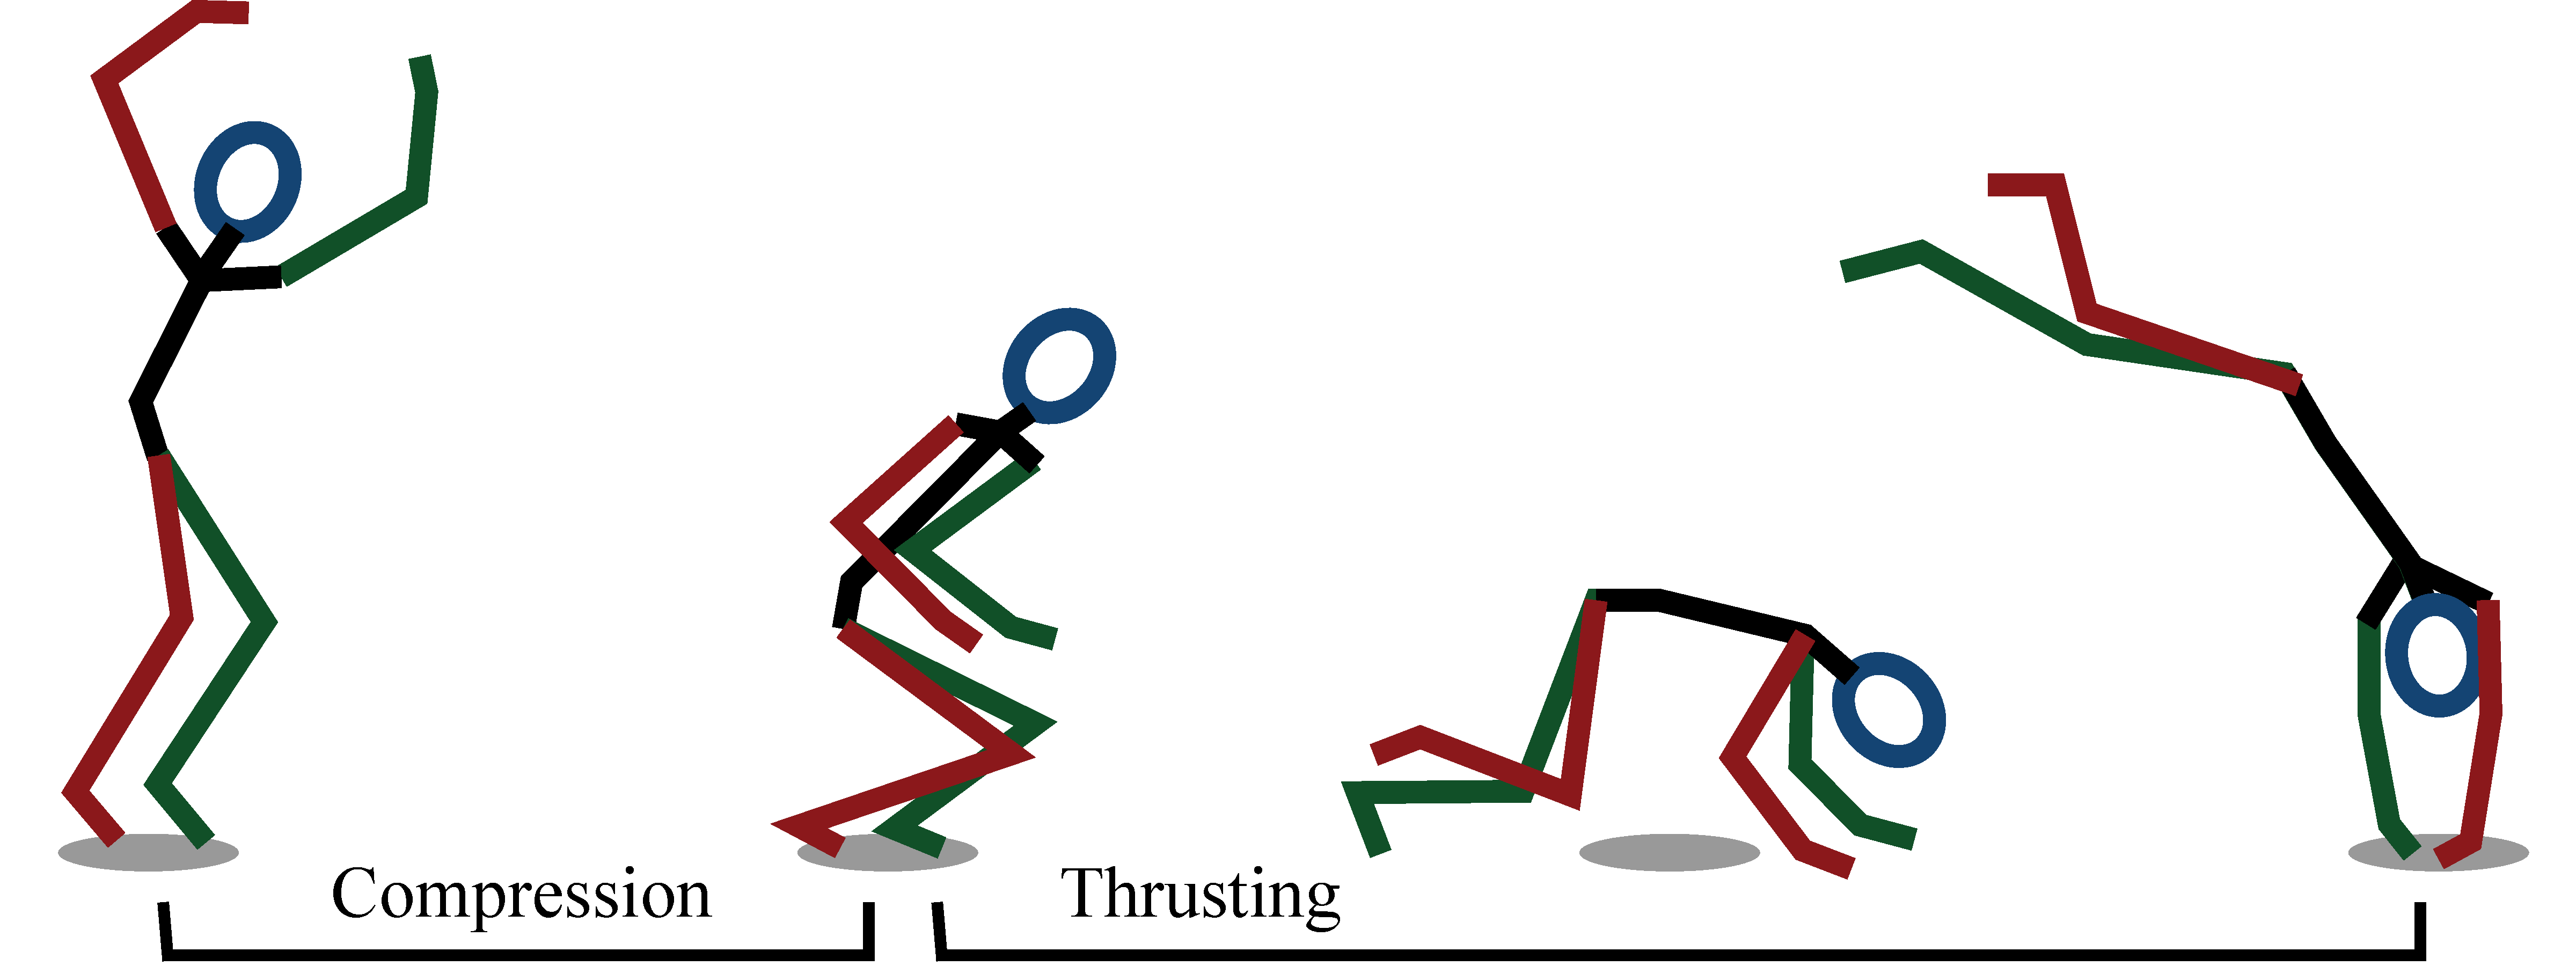
\includegraphics[width=4.2in]{images/feet-first}
\caption{Two-step impact stage for the feet-first strategy.}
\label{fig:landing_feet-first}
%% \end{minipage}
%% \begin{minipage}{0.1\textwidth}
%% 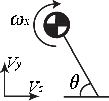
\includegraphics[width=0.8in]{images/COM}
%% \caption{}
%% \label{fig:COM}
%% \end{minipage}
\end{figure}
\ignorethis{
Our algorithm has two different landing styles for impact stage: 
\emph{Landing with hands} and \emph{Landing with feet}. They are not 
only different in the body parts for the first contact but also 
different in the strategies to control the trajectory of COM. While
\emph{Landing with hands} tries to achieve the desired forward momentum
at the lowest point of the COM, \emph{Landing with feet} divides the task
into two stages: compression and thrust. At the compression stages, 
the character acts like a damped spring to absorb all the velocities 
except the forward direction by crouching itself. When the COM reaches 
the bottom point, the algorithm enters the thrust stage and 
commands the character to kick the ground for the desired forward 
linear and angular momentum.}

\textbf{Virtual force.} The most important goal during the impact
stage is to stop the downward momentum before the character tragically
crashes into the ground. We do so by applying virtual forces to
control the vertical position and velocity of the COM. In addition,
our algorithm favors virtual forces that result in temporally smooth
ground reaction forces to distribute the impact evenly over
time. \ignorethis{in hopes of avoiding large joint stress at all
  times.} With these control goals, our algorithm aims to
use constant acceleration of the COM to achieve the desired COM
position $\bar{c}_y$ and velocity $\bar{\dot{c}}_y$ from the current
state ($c_y$ and $\dot{c}_y$).
\begin{equation}
\label{eqn:landing_controlY}
\ddot{c}_y = \frac{1}{2}(\bar{\dot{c}}_y^2 - \dot{c}_y^2) / (\bar{c}_y-c_y)
\end{equation}
A virtual force of $-m\ddot{c}_y$ in the vertical direction is then evenly
distributed to the end-effectors that are in contact with the ground.

Virtual forces in the horizontal direction are important to achieve
the desired forward linear momentum and angular momentum at the end of 
compression, or to achieve the desired forward thrust for the feet-first
strategy. We use a simple feedback mechanism to compute the desired
horizontal acceleration of the COM.
\begin{equation}
\label{eqn:landing_controlXZ}
\ddot{c}_{x/z} = k_v (\bar{\dot{c}}_{x/z} - \dot{c}_{x/z})
\end{equation}
where $\bar{\dot{c}}_{x/z}$ is the desired COM velocity in forward and
lateral directions and $k_v$ is the damping coefficient. The
corresponding virtual force is distributed to the contacting
end-effectors inversely proportional to their distances to the
COM.

\begin{table}
\center
{
%% \small
\caption{Control parameters. 
}


\begin{tabular}{|c |c|c|c|c|c| }
\hline
\label{tab:landing_tracking}

& {\small Hip} & {\small Lower spine } & {\small Upper spine } & {\small Neck } & {\small Knee } \\ \hline 
\textbf{$k_p$} & {\small 90.0} & {\small 300.0}& {\small 180.0}& {\small 10.0} & {\small 60.0} \\ \hline 
\textbf{$k_d$} & {\small 20.0} & {\small 60.0} & {\small 40.0} & {\small  2.0} & {\small 13.0} \\ \hline


& {\small Ankle } & {\small Clavicle } & {\small Shoulder} & {\small Elbow } & {\small Wrist } \\ \hline 
\textbf{$k_p$} & {\small 15.0} & {\small 180.0}& {\small 120.0}& {\small 60.0} & {\small  9.0} \\ \hline
\textbf{$k_d$} & {\small  6.0} & {\small 40.0} & {\small 27.0} & {\small 13.5} & {\small  4.0} \\ \hline

%% \textbf{$k_p$} 
%% & {\tiny 90.0} & {\tiny 300.0}& {\tiny 180.0}& {\tiny 10.0} & {\tiny 60.0} 
%% & {\tiny 15.0} & {\tiny 180.0}& {\tiny 120.0}& {\tiny 60.0} & {\tiny  9.0} \\ \hline

%% \textbf{$k_d$} 
%% & {\tiny 20.0} & {\tiny 60.0} & {\tiny 40.0} & {\tiny  2.0} & {\tiny 13.0} 
%% & {\tiny  6.0} & {\tiny 40.0} & {\tiny 27.0} & {\tiny 13.5} & {\tiny  4.0} \\ \hline
%% \end{tabular}

%% \begin{tabular}{|c|c|c|c|c|c|}
\hline
{\small \textbf{$\bar{c}_y$} } &
{\small \textbf{$\bar{\dot{c}}_y$} } &
{\small \textbf{$\bar{\dot{c}}_{x/z}$} } &
{\small \textbf{$k_v$} } &
{\small \textbf{$k_p$} (Eq \ref{eqn:landing_controlRoll}) } &  
{\small \textbf{$\omega_{MAX}$} } \\ \hline

{\small 0.4m} & {\small 0.0m/s} & {\small 4.0m/s} & {\small 500} & {\small 800} & {\small 3.3 Rad/s} \\ \hline
\end{tabular}
}
\end{table}


\textbf{Joint tracking.} In addition to virtual forces, we use PID
servos to maintain joint angles of the torso and limbs that are not in
contact, while limbs in contact with the ground act like viscous
dampers (PID control with a zero spring coefficient). We also use PID
control to keep the chin tucked to reduce the chance of the head
impacting the ground. Please see Table \ref{tab:landing_tracking} for all the
parameters in our implementation. We set the constant integral gain
$k_i$ of contacting limbs as $50$, and $0$ for all other joints.



\subsection{Rolling Stage}
\label{sec:landing_rolling}
Once the character's COM passes the hand-ground contact area with
sufficient forward linear and angular momentum, rolling becomes a
relatively easy task. As long as the character is holding a pose with
a flexed torso, a reasonable rolling motion will readily carry out. If
the character wishes to land back on its feet and get up after
rolling, it must also maintain forward momentum and lateral balance
during the roll.

\textbf{Virtual force.} To this end, we apply a virtual force to guide
the horizontal position of the COM toward the feet area, while
restricting it above the support polygon formed by contact points. The
virtual force is applied on the character's hands so that it can use
the entire upper body to maintain momentum and
balance. The virtual force produces the desired acceleration of the COM 
computed using a feedback mechanism:
\begin{equation}
\label{eqn:landing_controlRoll}
\ddot{c}_{x/z} = k_p (\bar{c}_{x/z} - c_{x/z})
\end{equation}
where the desired position $\bar{c}$ is set to be the location of the
left foot.

\textbf{Joint tracking.} During rolling, the character tracks a simple
pose to tuck the head, flex the torso, and position the legs
appropriately. We treat legs asymmetrically to both facilitate
momentum control and improve the aesthetics of the motion. When the
character rolls on its back, it brings the left knee closer to the
chest and casually stretches the right leg. This arrangement helps the
character to regulate the angular velocity using the right leg while
getting ready to stand up on its left foot. Based on the forward
angular velocity at the beginning of the rolling stage, we adjust the
desired tracking angles for the right knee as:
\begin{equation}
\label{eqn:landing_controlLeg}
\theta_R = max( (1 - \omega_x / \omega_{MAX}) \pi, 0 )
\end{equation}
\ignorethis{
Our algorithm applies PD control on head,
torso and legs to track some desired joint angles. Head and torso are
bended in forward direction to make the back of the character round
for smooth rolling.  For controlling legs, we assign the different
tasks to left and right legs.  The left leg is always tightly tucked
toward torso and prepared for stand up.  On the other hand, the right
leg is relatively more stretched to regulate the inertia based on the
current angular velocity. For instance, the right leg is tightly
tucked in low speed and fully straightened in the opposite case. The
role of left and right legs can be swapped.
}
\subsection{Getting-Up Stage}
The last stage of landing phase is to stand up using the remaining
forward momentum. When the COM passes the foot contact, the character
will start to elevate its COM to a desired height.

\textbf{Virtual force.} Similar to previous stages, we again apply
virtual forces on the feet and the hands to control the vertical and
the horizontal positions of the COM respectively. We compute $\ddot{c}_y$
using the same formula from \secref{landing_impact} with different desired
height of the COM. For $\ddot{c}_{x/z}$, we use the same formula as
in \secref{landing_rolling}.

\textbf{Joint tracking.} During the getting-up stage, our algorithm
simply tracks the torso and the head to straighten the spine and untuck the chin.

\ignorethis{
\section{Landing Planner}
\label{sec:landingplanner}

\begin{figure}[ht]
\center
  \includegraphics[width=3.2in]{images/abstractmodel}
  \caption{Abstract Model for Landing Motion}
 \label{fig:landing_abstractmodel}
\end{figure}

The goal of landing planner is to guide COM for a smooth transition between 
airborne planner and rolling planner.
To illustrate the character at landing, we construct an abstract model which is 
a single point mass connected to the fixed contact point (Figure \ref{fig:landing_abstractmodel}).
In other words, it is similar to the inverted pendulum model with the varying length rod. 
To prepare rolling, we want to regulate the linear and angular velocity 
when the point mass is vertical to the contact point ($t = T_v$).
Since there are an infinite number of solutions, we assume 
the constant contact force $\vc{\bar{F}}_C$ to distribute the impact over time.

Therefore, our problem is finding the optimal landing orientation $\mat{R}_L$ 
and duration $T_v$ to achieve the desired linear and angular velocity, 
$\bar{\vc{v}}_{v}$ and $\bar{\vc{\omega}}_{v}$.
From the given $\mat{R}_L$ and the length between COM and the desired end-effectors $l_0$, 
we can calculate the position of COM at the landing $\vc{C}(0)$.
In the similar manner, we can obtain $\vc{C}(T_v)$ from the desired key-frame pose.
With the initial and final positions of COM, we can calculate the desired 
contact force $\vc{\bar{F}_C}$ by solving the following equation:

\begin{equation}
\label{eqn:landing_landingcom}
\vc{C}(T_V) = \vc{C}(0) + \vc{v}(0) T_v + \frac{\vc{\bar{F}}_C}{2m}T_v^2
\end{equation}

In fact, equation \ref{eqn:landing_landingcom} gives us the complete trajectory of COM.
Based on this, we can calculate the linear and angular velocity at time $T_v$.

\begin{eqnarray}
\vc{L}(T_v) = \vc{L}(0) + \int^{T_v}_{0} \vc{C}(t) \times \vc{\bar{F}}_C dt \\
\vc{v}(T_v) = \vc{v}(0) + \frac{\vc{\bar{F}}_C}{m}T_v \\
\vc{\omega}(T_v) = \mat{I}(T_v)^{-1} L(T_v)
\end{eqnarray}

We formulate the optimization for $\mat{R}_L$ and $T_v$
to minimize the difference between the velocity at $T_v$ and the desired velocity.

\begin{equation}
(\mat{R}_L^*, T_v^*) = \argmin_{\mat{R}_L, T_v} 
(w_0|\vc{v}(T_v) - \bar{\vc{v}}_{v}| + w_1|\vc{\omega}(T_v) - \bar{\vc{\omega}}_{v}|)
\end{equation}

Since the optimization problem is non-linear and non-differentiable, 
we apply a derivative free optimization algorithm to solve.
}
